\documentclass[a4, 12pt]{article}
\usepackage{graphicx}
\usepackage{hyperref}
\usepackage{datatool}
\usepackage{apacite}
\usepackage{dingbat}
\usepackage{subcaption}
\usepackage{wrapfig}
\usepackage{placeins}

\begin{document}
\section{Introduction}
\subsection{Motivation}
Inferring glacier thickness has been a long-standing problem for glaciologist. Acquiring such data today is often done with an airborne or sled-mounted ground penetrating radar. Such equipment can be costly and difficult to acquire, hence the development of inferring methods.\\

Determining mean ice thickness lets us estimate the total volume of ice in a given glacier, necessary to quantify the water stored. In the context of climate change, a proper estimate of ice thickness is necessary for correctly estimating sea-level change \cite{farinotti2016accurate}. Many techniques have been developed for this problem, such as "power law" or "scaling" methods, deriving total ice volume from glacier surface area \cite{bahr2015review}. Other more modern methods have been developed for inferring distributed ice thickness. Those methods, using theoretical and mathematical models, often need intricate and difficult assumptions such as uniform basal shear stress an estimation of basal velocity \cite{farinotti2016accurate}. A rapidly increasing number of models are being developed, hence the need of an accurate representation of their performance along various conditions. The Ice Thickness Models Intercomparison eXperiment \cite{farinotti2016accurate} or \textit{ITMIX} did exactly this. 17 models were compare in this extensive paper along 21 study sites. This study tremendously helped the development of a global estimate of distributed glacier thickness \cite{farinotti2019consensus}. The five best performing models out of the experiment needing easily available data were used to make this worldwide estimation. The modelled data is freely available online for glaciers across the world.\\

The goal of this article is to assess the accuracy of the global glacier thickness estimation over two study sites extensively studied by Andrew Nolan and Tryggvy Unnsteinsson. Ultimately, a model of the distributed ice thickness will be produced using the data learned from comparing the global ice thickness data with field measurements.

\section{Background}
\subsection{\textit{ITMIX}}
The Ice Thickness Models Intercomparison eXperiment \cite{farinotti2016accurate} is a project launched by the working group on glacier ice thickness estimation, part of the International Association of cryospheric sciences.\\
The experiment consists of 17 different models tested over 21 cases, providing at least, depending on data availability:
\begin{itemize}
\item a glacier outline (\textbf{GO}) 
\item a digital elevation model (\textbf{DEM})
\end{itemize}
And a combination of:
\begin{itemize}
\item the surface mass balance (\textbf{SMB})
\item the velocity field ($\boldsymbol{\vec{V}}$)
\item the rate of ice thickness change ($\boldsymbol{\frac{\partial h}{\partial t}}$)
\end{itemize}
% Need to get the actual sources for these
Four main types of models were outlined throughout the experiment, each needing specific data.
\begin{itemize}
	\item Minimization approaches
		\begin{itemize}
			\item Those models defines ice thickness inversion as a minimization problem. They use a cost 					function consisting of minimizing the difference between observed and modelled data. 	
		\end{itemize}
	\item Mass conserving approaches
		\begin{itemize}
			\item These methods are based on the principle of mass conservation \cite{farinotti2016accurate} The 						ice flux divergence has to be compensated by the rate of ice thickness change and the 						climatic mass balance:
				\[\nabla \cdot q = \frac{\partial h}{\partial t} - \dot{b}\]
		\end{itemize}
	\item Shear-stress based approaches
		\begin{itemize}
			\item Those approaches rely on some estimation of the basal shear stress $\tau$. They then 					solve for ice thickness using the shallow ice approximation (Fowler and Larson, 1978)
			\[h = \frac{\tau}{f\rho g \sin{\alpha}}\]
		\end{itemize}
	\item Velocity-based approaches
		\begin{itemize}
			\item The models described in this category are based on a form of Glen's flow law (Glen, 					1955) and an approximation of either the basal velocity $u_b$ or the depth-averaged profile 				velocity $\bar{u}$ from the surface velocity $u_s$.
		\end{itemize} 
	\item Other approaches
		\begin{itemize}
			\item GCneuralnet(Clarke et al., 2009) is a model based no artificial neural networks. It is based on the assumption that the bedrock topography resembles nearby unglaciarized valleys.
			\item Brinkerhoff (Brinkerhoff et al., 2016) is based on Bayesian inference. The idea is that the bed elevation and the ice flux divergence can be described as Gaussian random fields with known covariance but unknown mean.
		\end{itemize}		
\end{itemize}
The various needs of every type of the main categories of models was captured in table \ref{tab:itmix_models}. To note is that the table indicates the needs of the majority in the models presented, some use more data than the others in the same category.
\begin{table}[h!]
	\centering
	\caption{Models compared} \label{tab:itmix_models}
	\begin{tabular}{|c|c|c|c|c|c|}
	\hline
	Model&\textbf{GO}&\textbf{DEM}&\textbf{SMB}&$\boldsymbol{\vec{V}}$&$\boldsymbol{\frac{\partial h}{\partial t}}$\\
	\hline
	Minimization approach & \checkmark & \checkmark & \checkmark & \checkmark * & \\
	\hline
	Mass conservation approaches & \checkmark & \checkmark & & & \\
	\hline
	Shear-stress based approaches & \checkmark & \checkmark & & & \\
	\hline
	Velocity based approaches & \checkmark & \checkmark & & \checkmark & \\
	\hline
	GCneuralnet & \checkmark & \checkmark & & & \\
	\hline
	Brinkerhoff & \checkmark & \checkmark & \checkmark & \checkmark & \checkmark \\
	\hline
	\end{tabular}
	\\
	\footnotesize A \checkmark with an asterix means that the model can make use of the data but it is not needed.\\
\end{table}
\\
\textit{ITMIX} ranked the models from best to worst according to their performance over two rankings:
\begin{itemize}
	\item Their performance over the glaciers they tested.
	\item Their performance over all the glaciers, considering the amount of test-cases. 
\end{itemize}
One of the main conclusions out of \textit{ITMIX} is that more data do not necessarily mean a better model. This is probably caused by the high variation in the methodology used by various scientists to capture such data.\\As there is limited data available for our study sites, it is important to choose a model corresponding to potentially accessible data. The findings of \textit{ITMIX} confirms that the lack of surface velocity field or rate of ice thickness change over time data isn't too dramatic.
\section{Study sites}
\subsection{Job glacier}
\subsubsection{Site description}
% I think I need more information on the location and the history of the place. I'll go further into detail by reading more of Tryggvi's thesis proposal.
\begin{figure}[h!]
\centering
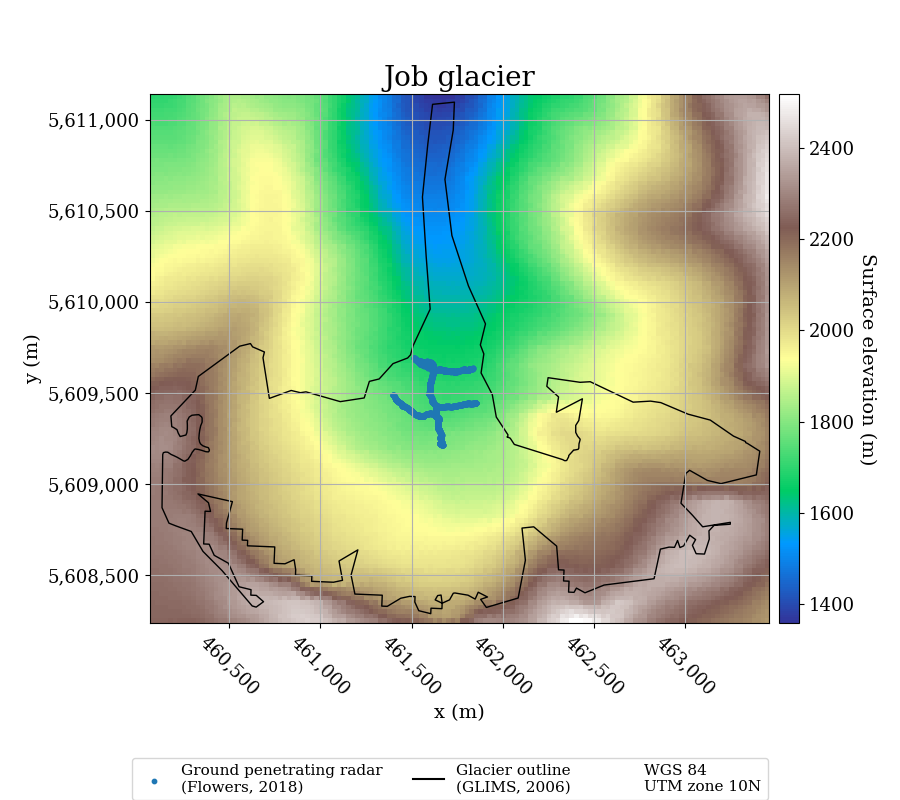
\includegraphics[scale=0.5]{../job_kluane_maps/Job glacier_elevation.png}
\caption{Job glacier's elevation}
\label{fig:job_dem}
\end{figure}
% Is the landslide section pertinent? I understand that it is not in Tryggvi's main research focus, but it helps motivating the glacier flow model and the ice thickness
Job glacier is located upon Mt. Meager, a volcano in southwestern British Columbia. This glacier, like most glaciers across the world, has seen a net negative mass balance in the last ten years \cite{reyes2004stratigraphic}. This decreasing amount of ice means increasing amounts of water flowing along Mt. Meager. In 2010, this caused the largest reported landslide in the history of Canada happened upon Mt. Meager's south flank \cite{roberti2018landslides}.\\
Fumaroles emerged from the surface of the glacier in 2016. \citeauthor{roberti2018landslides} \citeyear{roberti2018landslides} states that the fumarolic activity has probably been active for a long period, but only recorded from the thinning of the glacier.\\
The research covered by Tryggvi Unnsteinsson aims to understand the dynamical interaction between the glaciological and volcanic systems upon Mt. Meager and the glaciological conditions required for fumarole emergence.
\subsubsection{Data available} % Should we move these subsection into another section after the model section?
The data available for this study site consists of a 1 $m^2$ resolution LIDAR from (?), a glacier outline from Randolph Glacier Inventory and ice thickness measurements from a ground penetrating radar campaign held by Dr. Flowers and her team in September 2018. The ice thickness measurements only cover a small portion of the glacier and the point data can be seen on figure \ref{fig:job_dem}.\\
\FloatBarrier
\subsection{Little Kluane glacier}
\begin{figure}[h!]
\centering
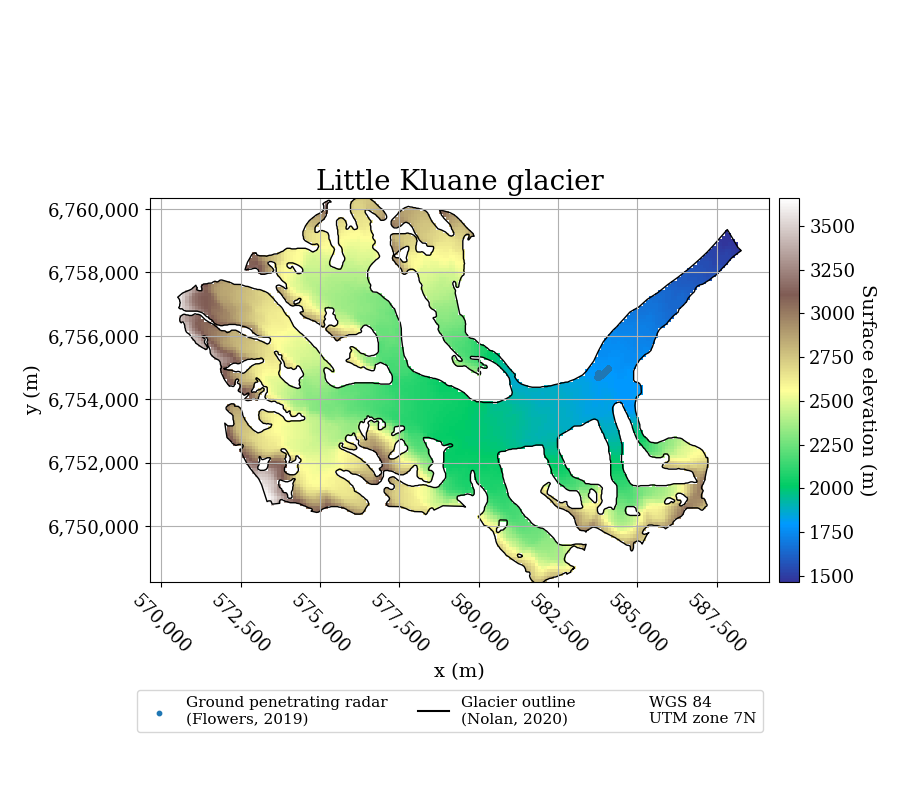
\includegraphics[scale=0.5]{../job_kluane_maps/Little Kluane glacier_elevation.png}
\caption{Little Kluane glacier's elevation}
\label{fig:lk_dem}
\end{figure}
The little Kluane glacier is the nickname given to a small surging glacier part of the bigger Kluane glacier, located in the Kluane national park and reserve, in the St. Elias moutains of Yukon. More stuff need to be said.
\subsubsection{Data available}
The data available for this study site consists of a DEM we need to find (potentially DEM Arctic v2?)other than the one used by the global thickness model, a glacier outline from Nolan (2020) and ice thickness measurements from a ground penetrating radar campaign held by Dr. Flowers and her team in (??). The ice thickness measurements only cover a small portion of the glacier and the point data can be seen on figure \ref{fig:lk_dem}.
\section{The global consensus estimate: assessing the error}
Following \textit{ITMIX}, \citeauthor{farinotti2019consensus} bettered the earlier global estimate from \citeauthor{huss2012distributed} \citeyear{huss2012distributed}. In this paper, they use findings from \textit{ITMIX} to infer ice thickness of all the glaciers around the globe. using five different models and weighting each of their results to minimize the error. The computed models are freely available online and this raises a question: if we already have an estimate of ice thickness for our study sites, why should we compute one ourselves?\\ Having real world ice thickness measurement data can help us better the approximation made by \citeauthor{farinotti2019consensus} \citeyear{farinotti2019consensus}. First, we need to assess the error in those models by comparing it to our point data.
\subsection{Job glacier}
% Figure needs some tinkerink, would be great to have independant maps instead of together finally eh
The ice thickness model from \citeauthor{farinotti2019consensus} \citeyear{farinotti2019consensus} can be seen in figure \ref{fig:job_thickness}.
\begin{figure}[h!]
\centering
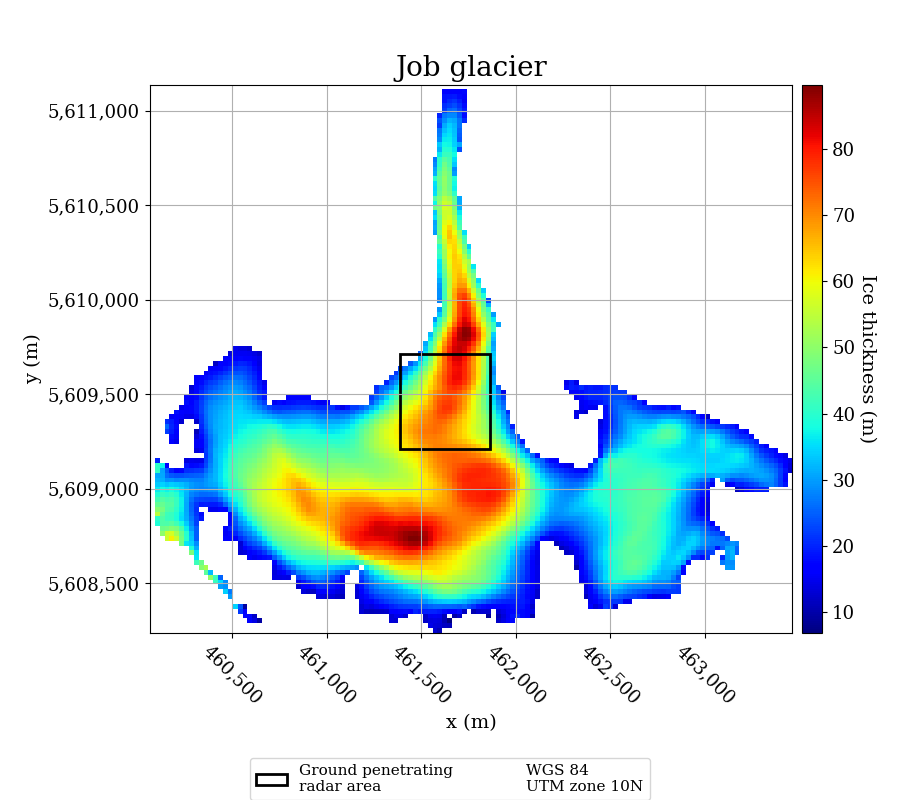
\includegraphics[scale=0.45]{../job_kluane_maps/Job glacier_thickness.png}
\caption{The modelled thickness of Job glacier}
\label{fig:job_thickness}
\end{figure}
\\
The modelled distributed ice thickness puts the thinner ice upon the higher elevations and the thicker ice in the lower areas, all the way down the flow path of the glacier. Also shown on figure \ref{fig:job_thickness} is the area covered by the ground penetrating radar point data. We can see the comparison between the field and modelled data on figure \ref{fig:cropped_job_thickness}.
\begin{figure}[h!]
\centering
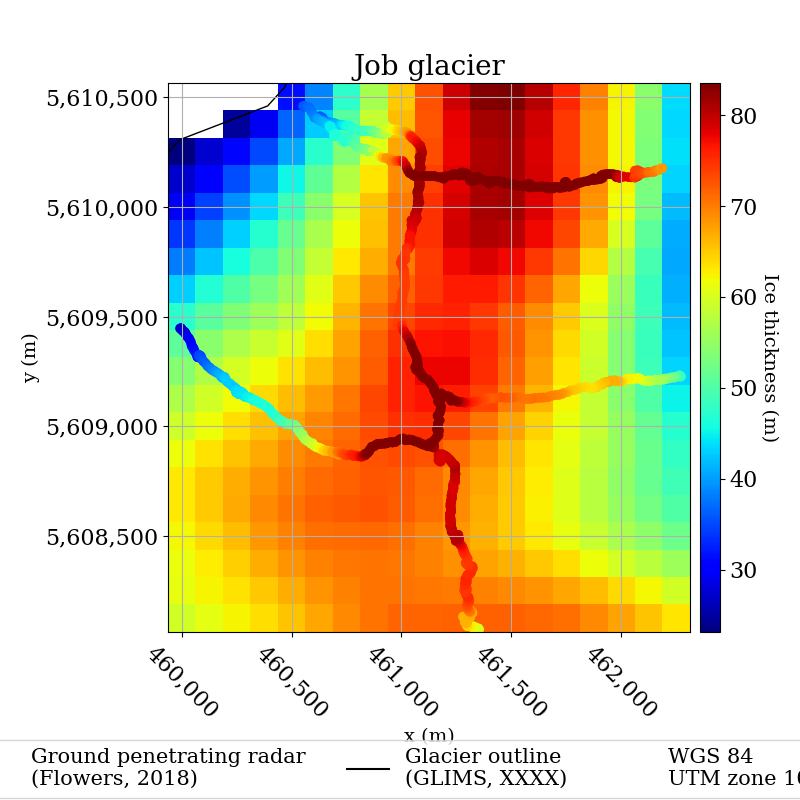
\includegraphics[scale=0.45]{../job_kluane_maps/Job glacier_cropped_thickness.png}
\caption{The field and modelled thickness data of Job glacier}
\label{fig:cropped_job_thickness}
\end{figure}
A higher discrepancy seem to be located upon the margin of the glaciers, modelling thicker ice to the west margin and shallower ice to the east margin. To compute the error \[\Delta h = h' - h\] we need to transform our point data to pixel data. As we have more points than pixels, the mean value of the point thickness data is taken for each cell. The computed error is shown in figure  \ref{fig:error_job_thickness}.
\begin{figure}[h!]
\centering
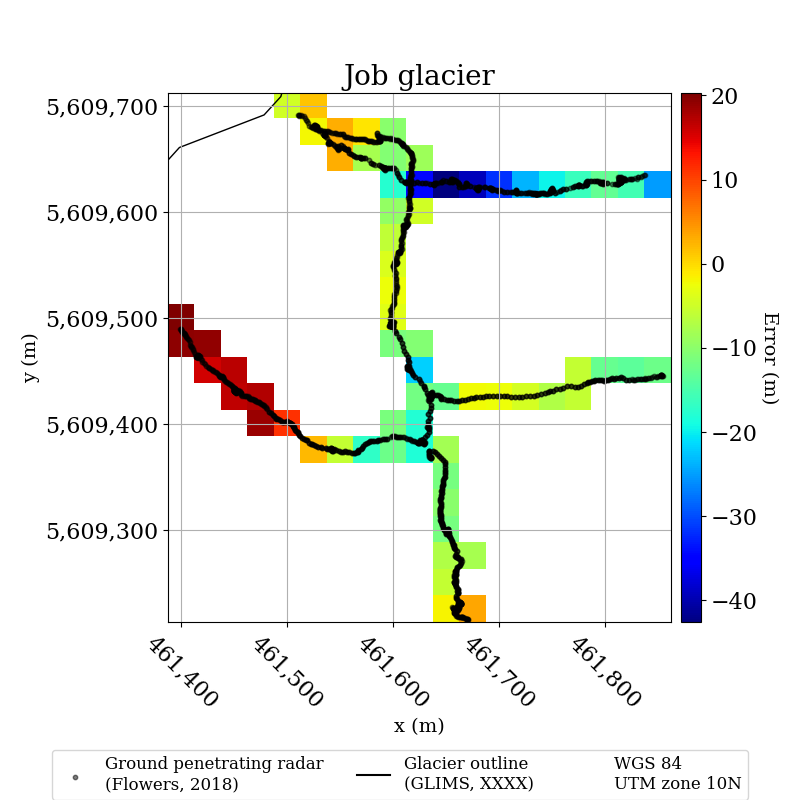
\includegraphics[scale=0.4]{../job_kluane_maps/Job glacier_error.png}
\caption{The error in Job glacier's model}
\label{fig:error_job_thickness}
\end{figure}
The positive and negative error in the western and eastern margin respectively seems to be because the model doesn't take into account the glacier's flow direction. There might be thicker ice in the eastern region because of the curved nature of the flow line (??). It is also possible to compute the relative distributed error: \[\delta h = \frac{h' - h}{h} = \frac{\Delta h}{h}\]
This relative error is shown in a similar manner on figure \ref{fig:rel_error_job_thickness}. The error is shown in percentage for convenience.
\begin{figure}[h!]
\centering
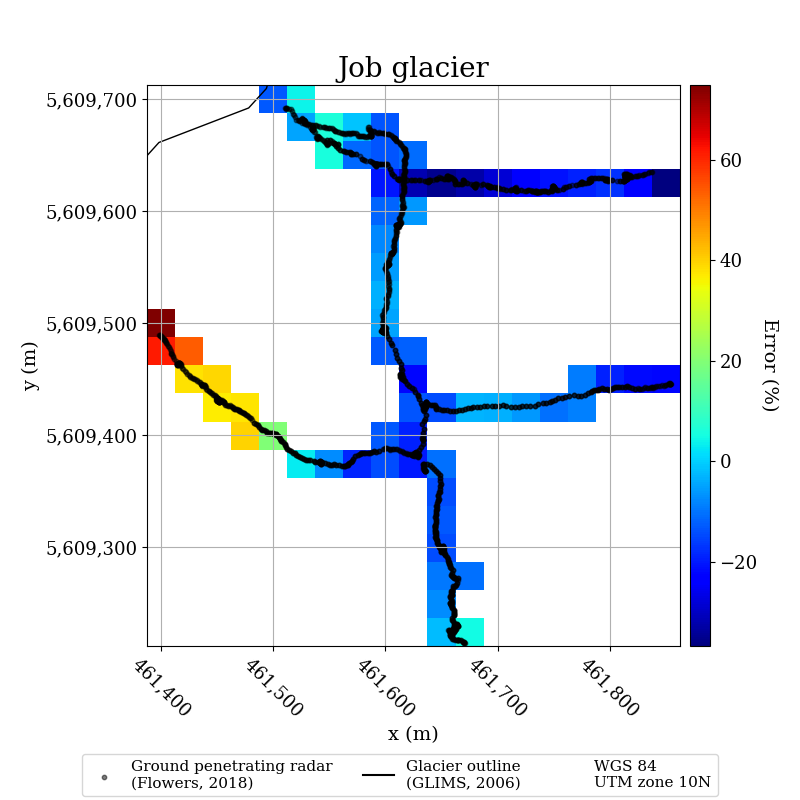
\includegraphics[scale=0.4]{../job_kluane_maps/Job glacier_rel_error.png}
\caption{The relative error in Job glacier's model}
\label{fig:rel_error_job_thickness}
\end{figure}
\\
Plotting the mesured thickness on the x-axis and their corresponding modelled thickness on the y-axis gives us a scatter plot showing the overall error distribution. Such a plot is shown on figure \ref{fig:xy_job_thickness}. If the modelled and measured thickness were identical, they'd be lying upon the $x=y$ line. In Job glacier's case, they seem to be distributed over the line for the shallower measurements and farther under the line for the thicker measurements. 
\begin{figure}[h!]
\centering
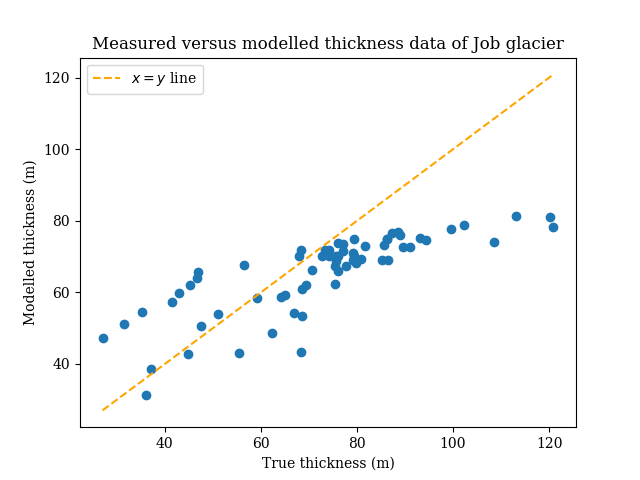
\includegraphics[scale=0.5]{../job_kluane_maps/Job glacier_xy.png}
\caption{The measured and modelled thickness of Job glacier}
\label{fig:xy_job_thickness}
\end{figure}
\subsection{Little Kluane}
Similar plots were made for the Little Kluane glacier. The ice thickness model from \citeauthor{farinotti2019consensus} \citeyear{farinotti2019consensus} can be seen in figure \ref{fig:lk_thickness}.
\begin{figure}[h!]
\centering
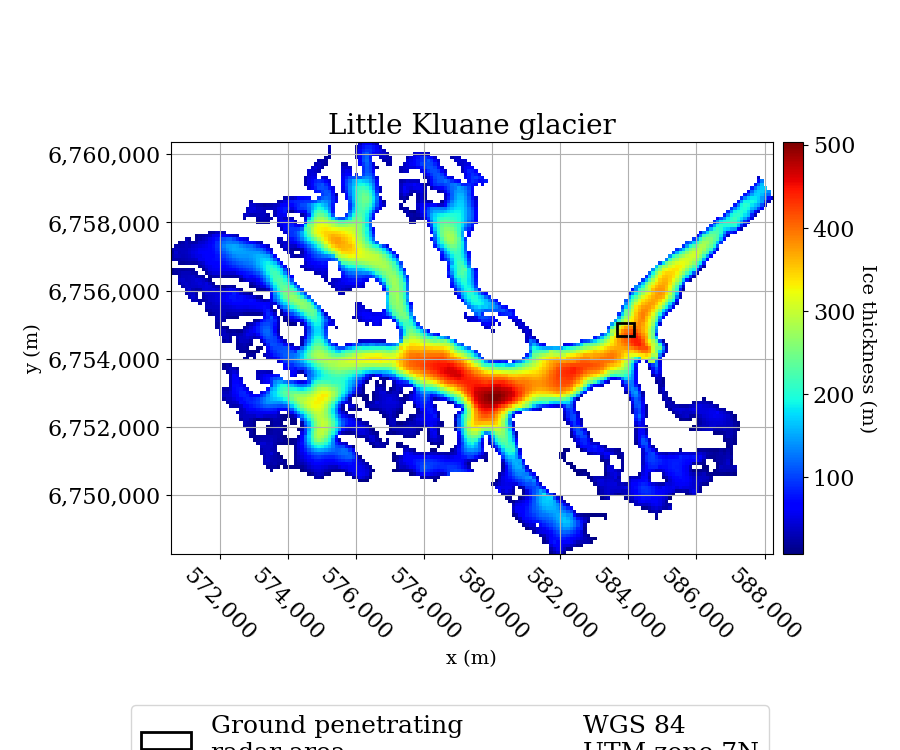
\includegraphics[scale=0.4]{../job_kluane_maps/Little Kluane glacier_thickness.png}
\caption{The modelled thickness of Little Kluane glacier}
\label{fig:lk_thickness}
\end{figure}
\\
Little Kluane being a bigger glacier than Job, the absolute thickness is much greater. The modelled distributed thickness puts the thicker ice in the lower areas, along the flow lines. Figure \ref{fig:lk_thickness} also shows the area covered by the ground penetrating radar data. Because the data was taken during its surge, it was difficult for the team to cover a great section without having to cross crevasses, hence the smaller area shown for Little Kluane. In a similar manner to the precedent section, the ice thickness is shown on figure \ref{fig:cropped_lk_thickness}.
\begin{figure}[h!]
\centering
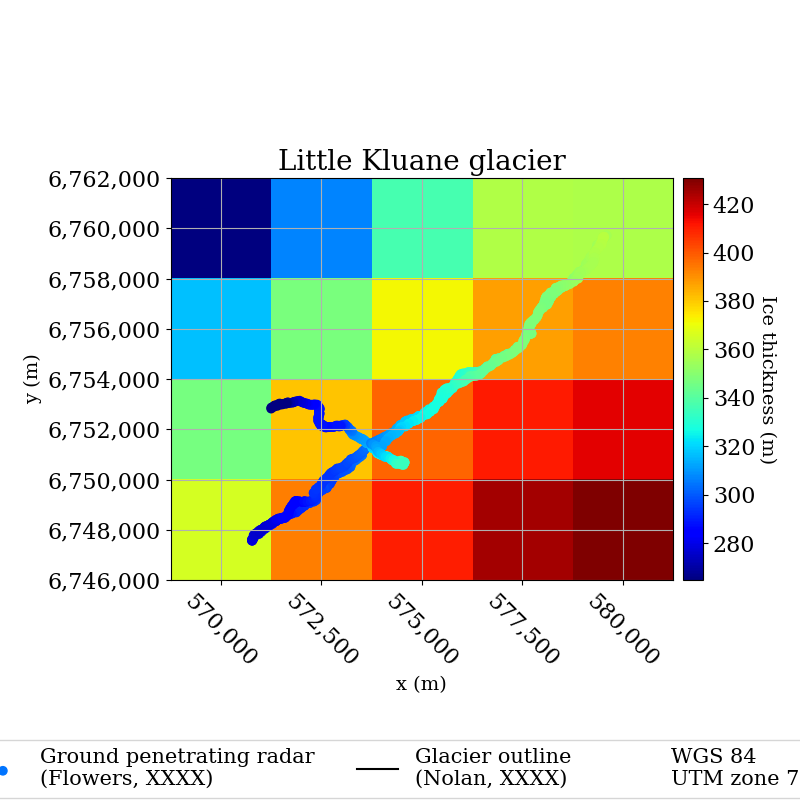
\includegraphics[scale=0.4]{../job_kluane_maps/Little Kluane glacier_cropped_thickness.png}
\caption{The modelled thickness of Little Kluane glacier}
\label{fig:cropped_lk_thickness}
\end{figure}
It is hard to discern any  pattern in this case, but the error is positive overall. From the single cross section line, is is possible to deduce that the ice is probably much thinner at the extremities. The computed error and relative error are shown on figures \ref{fig:error_lk_thickness} and \ref{fig:rel_error_lk_thickness}.
\begin{figure}[h!]
\centering
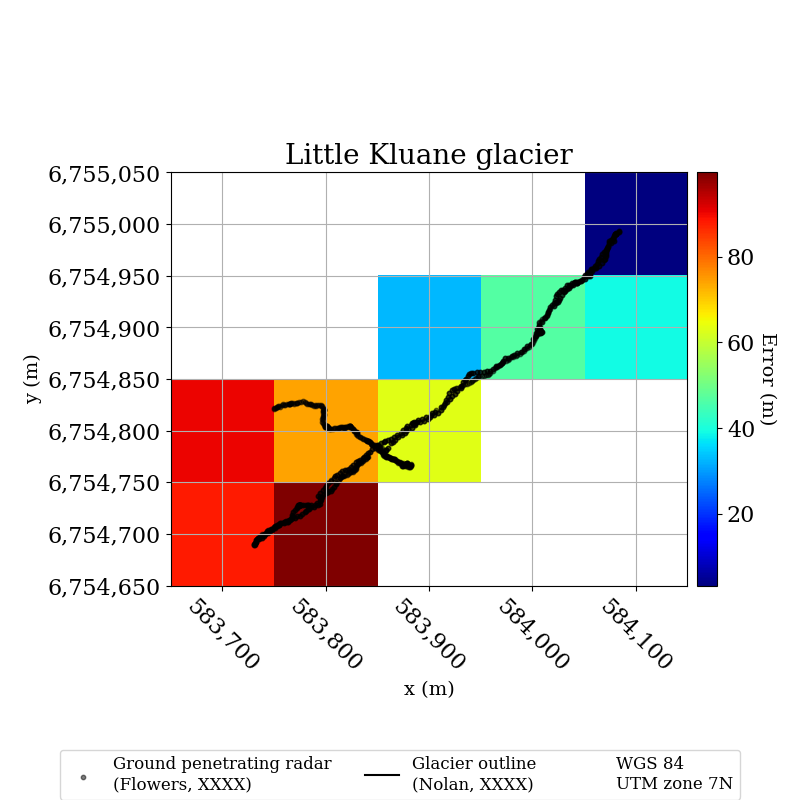
\includegraphics[scale=0.4]{../job_kluane_maps/Little Kluane glacier_error.png}
\caption{The error in Little Kluane glacier's model}
\label{fig:error_lk_thickness}
\end{figure}
\\
\begin{figure}[h!]
\centering
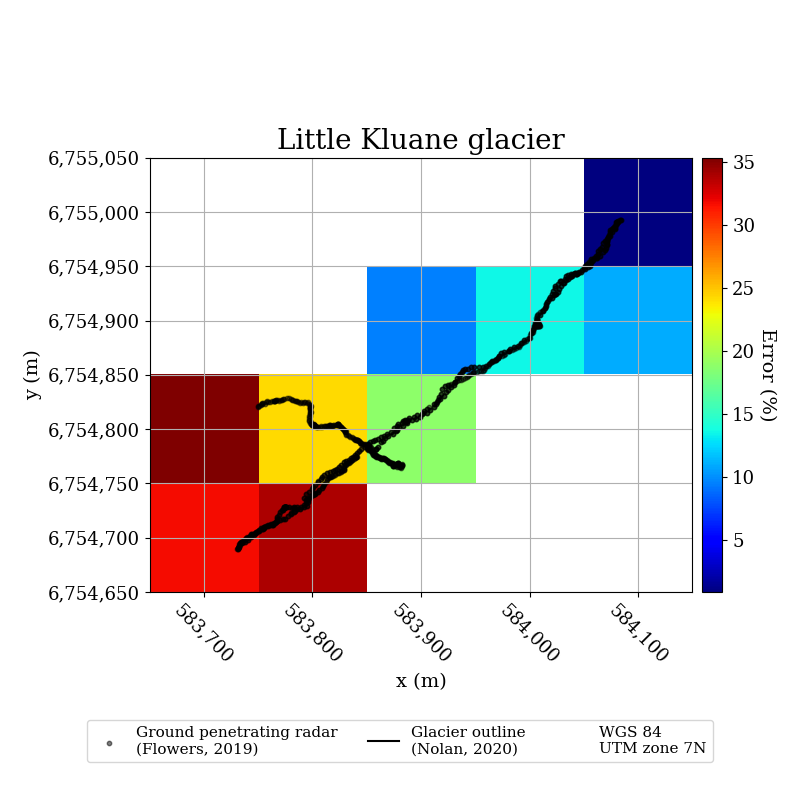
\includegraphics[scale=0.4]{../job_kluane_maps/Little Kluane glacier_rel_error.png}
\caption{The relative error in Little Kluane glacier's model}
\label{fig:rel_error_lk_thickness}
\end{figure}
\\
One thing very important to note is the surging nature of the glacier at the times of measurements and the unknown time period covered by the modelled data. The paper coming out in 2019 and the glacier surging in 2018, it is unlikely but possible that they used data from after the surge. More info is needed on this and it is very important.
\\
Similarly to Job glacier, the corresponding measured and modelled ice thickness data is shown on a scatter plot on figure \ref{fig:xy_lk_thickness}. The figure shows us that the error is strictly positive.
\begin{figure}[h!]
\centering
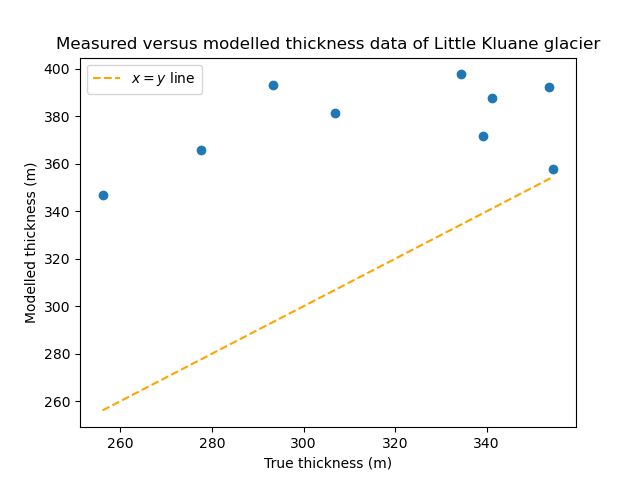
\includegraphics[scale=0.5]{../job_kluane_maps/Little Kluane glacier_xy.png}
\caption{The measured and modelled thickness of Little Kluane glacier}
\label{fig:xy_lk_thickness}
\end{figure}
\subsection{Error data}
The errors between the modelled and observed data from Job and Little Kluane was computed and their main statistics is shown in table \ref{tab:error_table}. Box plots of both  the error and the relative error also have been produced and are visible in figure \ref{fig:job_lk_boxplot}.

% Load data from the error csv %
\DTLloaddb{errdata}{../job_kluane_maps/data.csv}

\begin{table}[h!]
\centering
\small
\caption{Error data from Job and Little Kluane}
\label{tab:error_table}
\noindent\makebox[\textwidth]{
\begin{tabular}{|c|c|c|c|c|c|c|c|}
\hline
% Header %
\textbf{Glacier} & \textbf{Mean} & \textbf{Std} & \textbf{Median} & \textbf{Max} & \textbf{Absolute mean} & $\boldsymbol{MSE}$
% Iterated csv data %
\DTLforeach{errdata}
		{\glacier=Glacier,\mean=Mean,\std=Std,\med=Median,\abs=Absolute mean,\mse=Mean square, \max=Maximum}
{\\ \hline \glacier & \mean & \std & \med & \max & \abs & \mse}
\\ \hline
\end{tabular}
}
\footnotesize $MSE$ is the mean square error, computed as $\frac{1}{n}\sum(\Delta h)^2$, where $n$ is the number of cells.
\end{table}
% Load box plots %
\begin{figure}[h!]
\makebox[\textwidth][c]{
\begin{subfigure}{0.7\textwidth}
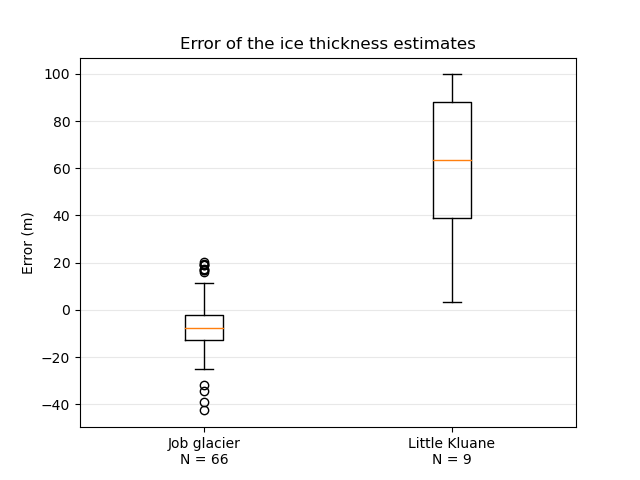
\includegraphics[width=\linewidth]{../job_kluane_maps/boxplots.png}
\caption{Error}
\label{fig:box_plot_error}
\end{subfigure}
\begin{subfigure}{0.7\textwidth}
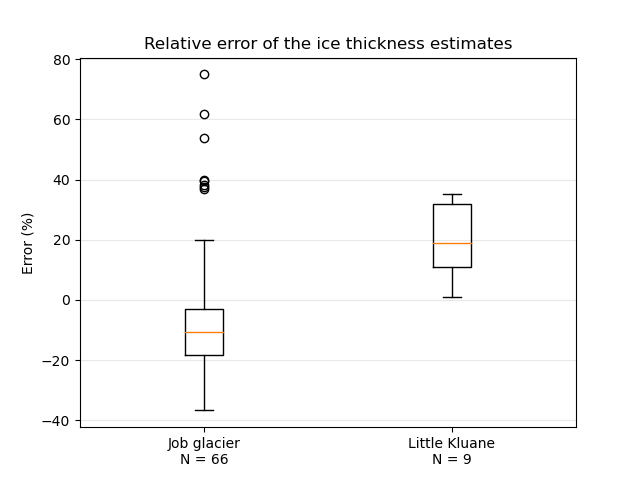
\includegraphics[width=\linewidth]{../job_kluane_maps/rel_boxplots.png}
\caption{Relative error}
\label{fig:box_plot_rel_error}
\end{subfigure}
}
\caption{Error box plots for Job and Little Kluane glaciers}
\label{fig:job_lk_boxplot}
\end{figure}
\FloatBarrier

This confirms us that, for Job glacier's case, the mean error is negative meaning that the ice thickness is mostly underestimated. The percentage standard deviation is however significant (In what way? How is that an absolute metric?) We do see however a few outliers on the box plot, showing that in some areas the thickness is greatly overestimated, up to 80\%. This error is located in the western margin of the glacier which is the concave section of the flow line.

For Little Kluane glacier, the error is strictly positive, meaning that the ice thickness is over estimated for every point measured. The model also shows less variation than in Job's case with a smaller percentage standard deviation.

These findings validate the need to better the model with the ice thickness measurements.

\bibliographystyle{apacite}
\bibliography{References}

\end{document}